\documentclass{estilo}
\usepackage[spanish]{babel}
\usepackage{graphicx}
\usepackage{float}
\usepackage{amsmath}        % para los vectores columnas
\usepackage{amsfonts}       % para las negrita de pizarra
\usepackage{amssymb}        % para simbolos matematicos
\usepackage{hyperref}       % para utilizar referencias
\usepackage{multirow}       % para las tablas
\usepackage{dsfont}
\usepackage{listings}
\usepackage{tabularx}
\usepackage{colortbl}
\usepackage{xcolor}
\usepackage{booktabs}
\hypersetup{
    colorlinks=true,
    urlcolor=blue,
    linkcolor=black,
    citecolor=black
}
\usepackage{xurl}
\definecolor{codegreen}{rgb}{0,0.6,0}
\definecolor{codegray}{rgb}{0.5,0.5,0.5}
\definecolor{codepurple}{rgb}{0.58,0,0.82}
\definecolor{backcolour}{rgb}{0.95,0.95,0.92}

% ==========================================
% SOLUCIÓN ADVERTENCIA FANCYHDR
% ==========================================
\setlength{\headheight}{30pt} 

% ==========================================
% DEFINICIÓN DE COLORES DEL PROYECTO
% ==========================================
% Paleta SocioUnido Base (Acromática)
\definecolor{suNegro}{HTML}{111111}
\definecolor{suGrisOscuro}{HTML}{4A4A4A}
\definecolor{suGrisClaro}{HTML}{F5F5F5}
\definecolor{suBlanco}{HTML}{FFFFFF}

% Paleta Adaptativa: C. A. Boca Juniors
\definecolor{bocaAzul}{HTML}{003893}
\definecolor{bocaOro}{HTML}{F2A900}

% Paleta Adaptativa: C. A. San Lorenzo de Almagro
\definecolor{caslaAzul}{HTML}{002F6C}
\definecolor{caslaRojo}{HTML}{C8102E}

% Paleta Adaptativa: C. A. Talleres de Remedios de Escalada
\definecolor{talleresRojo}{HTML}{E30613}

% ==========================================
% DEFINICIÓN DEL COMANDO FALTANTE
% ==========================================
\newcommand{\muestra}[1]{\raisebox{-0.4ex}{\fcolorbox{black}{#1}{\hspace{1.2em}\vrule height 1.2ex width 0pt}}}

\lstdefinestyle{mystyle}{
    backgroundcolor=\color{backcolour},   
    commentstyle=\color{codegreen},
    keywordstyle=\color{magenta},
    numberstyle=\tiny\color{codegray},
    stringstyle=\color{codepurple},
    basicstyle=\ttfamily\footnotesize,
    breakatwhitespace=false,         
    breaklines=true,                 
    captionpos=b,                    
    keepspaces=true,                 
    numbers=left,                    
    numbersep=5pt,                  
    showspaces=false,                
    showstringspaces=false,
    showtabs=false,                  
    tabsize=2
}
\lstset{style=mystyle}

\usepackage{enumitem,multicol,setspace}
\newcounter{subenum}[enumi] % para las multicolumnas
\renewcommand{\thesubenum}{\arabic{subenum}}
\usepackage[nomessages]{fp}
\FPeval\thecolwidth{round(1/4:4)}% Specify number of columns -> column width
\newcommand{\newitem}[1]{%
  \refstepcounter{subenum}%
  \parbox{\dimexpr\thecolwidth\linewidth-.5\columnsep}{%
    \makebox[\labelwidth][r]{(\thesubenum)\hspace*{\labelsep}}%
    #1}\hfill%
}

\usepackage{scalerel,stackengine} % para el sombrero
\stackMath
\newcommand\rhat[1]{%
\savestack{\tmpbox}{\stretchto{%
  \scaleto{%
    \scalerel*[\widthof{\ensuremath{#1}}]{\kern-.6pt\bigwedge\kern-.6pt}%
    {\rule[-\textheight/2]{1ex}{\textheight}}%WIDTH-LIMITED BIG WEDGE
  }{\textheight}% 
}{0.5ex}}%
\stackon[1pt]{#1}{\tmpbox}%
}
\parskip 1ex

\usepackage{mathtools}      % floor y ceil
\DeclarePairedDelimiter\ceil{\lceil}{\rceil}
\DeclarePairedDelimiter\floor{\lfloor}{\rfloor} 

\usepackage[style=authoryear-comp]{biblatex}


\begin{document}

% ==============================================================================
% FICHA EJECUTIVA - SOCIOUNIDO
% ==============================================================================

\begin{center}
    \LARGE \textbf{Ficha Ejecutiva del proyecto} \\
    \vspace{0.2cm}
    \large Trabajo Profesional de Ingeniería en Informática $\cdot$ Kit de lectura del jurado
\end{center}
\vspace{0.3cm}

% --- BLOQUE DE IDENTIFICACIÓN ---
\noindent
\renewcommand{\arraystretch}{1.5}
\begin{tabularx}{\textwidth}{|>{\columncolor[gray]{0.95}\bfseries}p{4.5cm}|X|}
\hline
Título del proyecto & SocioUnido: Plataforma inteligente que centraliza la gestión administrativa de los clubes, optimizando el uso de espacios compartidos, previniendo la morosidad y asegurando los accesos al estadio. \\
\hline
Modalidad & Cursada (Práctica Profesional Supervisada - Empresas de Base Tecnológica 2) \\
\hline
Integrantes del equipo & 
Ascencio, Felipe Santino -- 110675 \newline
Ghosn, Lautaro Gabriel -- 106998 \newline
Guerrero, Martín -- 107774 \newline
Zielonka, Axel -- 110310 \\
\hline
Director / co-Director & Mg. Ing. Gabriel Piñeiro / Ing. Agustín Perrotta \\
\hline
Orientador en el campo de desempeño & Franco Di Mauro -- Profesor Adjunto de la materia Empresas de Base Tecnológica II (Facultad de Ingeniería, Universidad de Buenos Aires) \\
\hline
Informe Final al que corresponde & Versión Final -- Agosto 2026. \\
\hline
Fecha de esta Ficha & 26/08/2026 \\
\hline
\end{tabularx}

\vspace{0.3cm}

% --- 1. ABSTRACT GRÁFICO ---
\section*{1. Abstract gráfico}

\begin{figure}[H]
    \centering
    % Se asume que la imagen está en la ruta especificada en el ZIP de LaTeX importado
    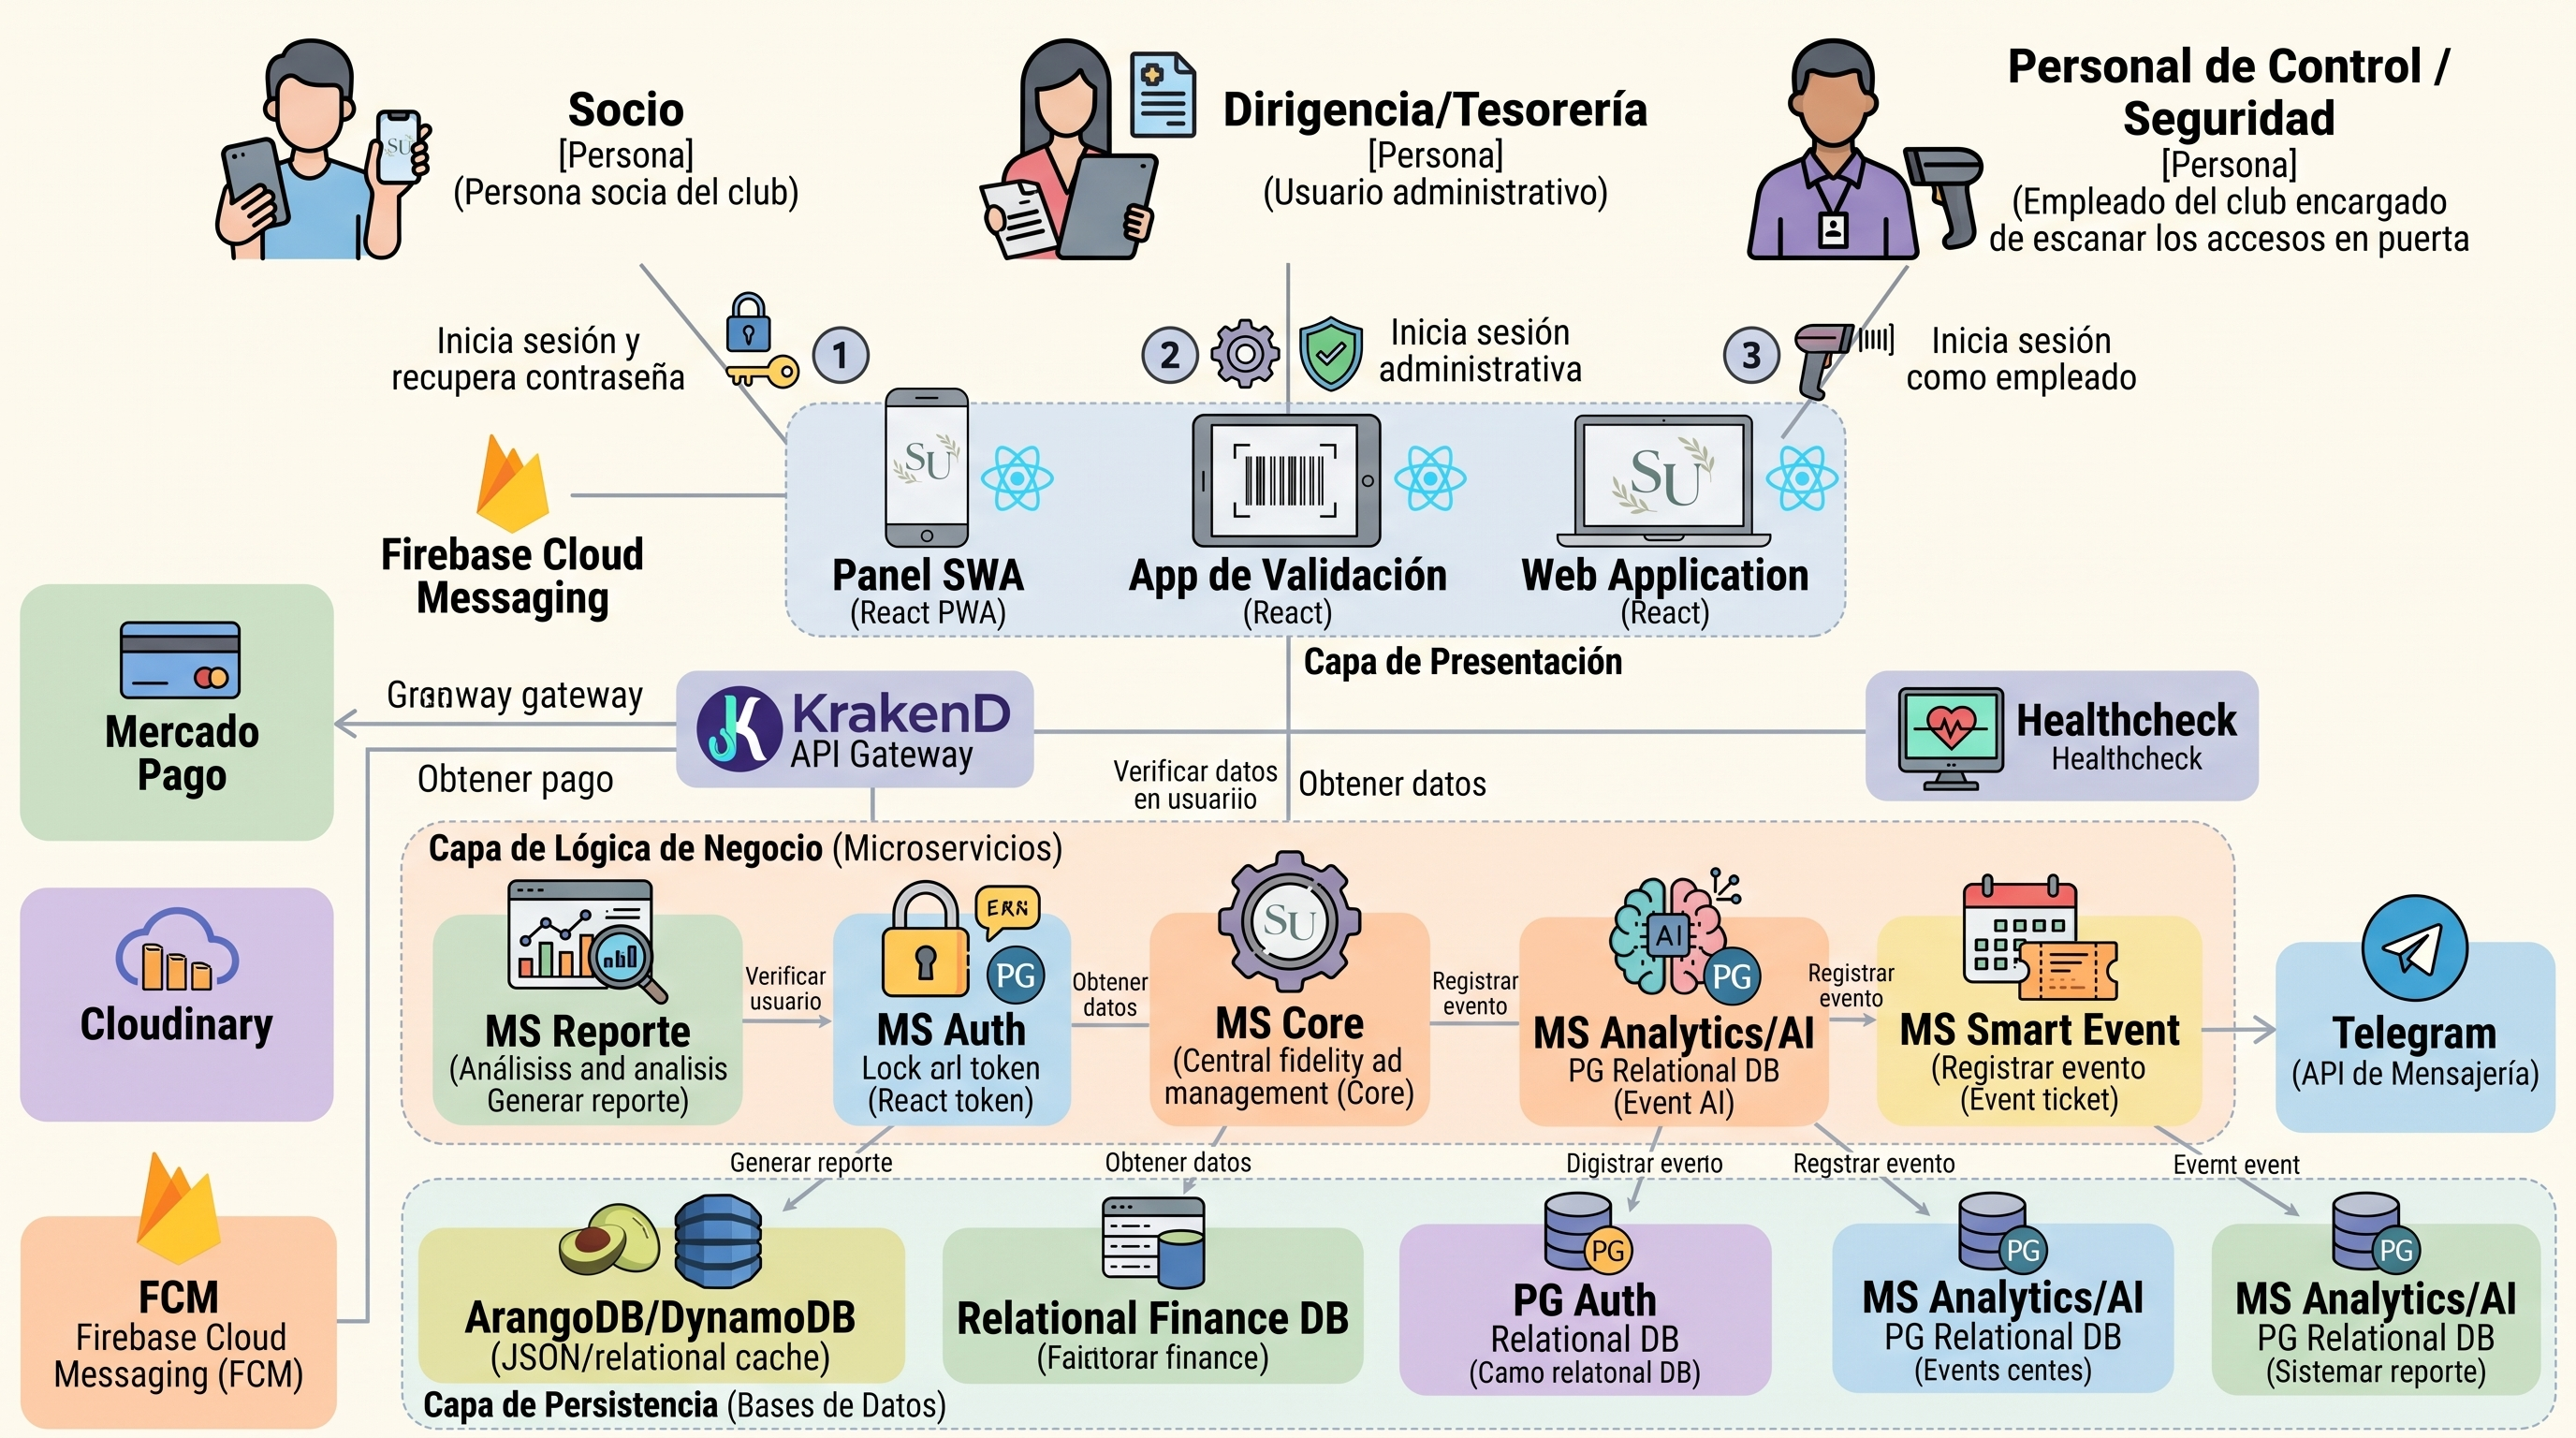
\includegraphics[width=\textwidth]{img/arquitectura/c2_componentes.jpg}
    \caption{Diagrama de Contenedores (C2) de SocioUnido. Ilustra la arquitectura orientada a microservicios, el aislamiento de las interfaces frontend respecto a la capa de lógica de negocio, centralizada bajo un API Gateway, y su integración con pasarelas de terceros.}
    \label{fig:abstract_grafico}
\end{figure}

\vspace{0.5cm}

% --- 2. MATRIZ DE CONTRIBUCIONES Y RESULTADOS ---
\section*{2. Matriz de Contribuciones y Resultados}

\noindent
\renewcommand{\arraystretch}{1.4}
\begin{tabularx}{\textwidth}{|>{\raggedright\arraybackslash}p{3.5cm}|>{\raggedright\arraybackslash}X|>{\raggedright\arraybackslash}p{3.5cm}|>{\raggedright\arraybackslash}p{3cm}|}
\hline
\rowcolor[gray]{0.9}\textbf{Problema / Necesidad identificada} & \textbf{Solución de ingeniería implementada} & \textbf{Validación / Métrica obtenida} & \textbf{Responsable(s)} \\
\hline
Morosidad societaria crónica e ineficiencia en el recupero reactivo de cuotas impagas. & 
Integración con herramientas predictivas y digitalización de flujos de pago vía pasarela centralizada. & 
Detección temprana de socios en riesgo de abandono (\textit{churn rate}) y tableros proactivos operativos (\S 8.4.2 y \S 10.4.3). & 
Guerrero, Martín \newline Ghosn, Lautaro Gabriel \\
\hline
Colapso de redes móviles (4G/5G) en estadios masivos y fraude perimetral por préstamo de carnets físicos. & 
Módulo \textit{Smart Access} descentralizado basado en algoritmos criptográficos TOTP (\textit{Time-Based One-Time Password}). & 
Validación perimetral instantánea y 100\% \textit{offline}, mitigando el fraude sin requerir hardware costoso (\S 8.4.1 y \S 13.2). & 
Ghosn, Lautaro Gabriel \newline Zielonka, Axel \\
\hline
Alta fricción de descarga de aplicaciones (tasa de rebote) y barrera tecnológica en socios de diversas edades. & 
Implementación de un asistente conversacional omnicanal interactivo (BotIn) soportado por Procesamiento de Lenguaje Natural (PLN). & 
Interacción asíncrona sin fricción (Cero descargas) validada en flujos de consultas y cobros (\S 8.4.3 y \S 10.7). & 
Guerrero, Martín \newline Ascencio, Felipe Santino \\
\hline
Subutilización de infraestructura y pérdida de ingresos por ociosidad de activos compartidos. & 
Desarrollo de PWA adaptativa (marca blanca) con módulos de e-commerce y reservas digitales en tiempo real. & 
Despliegue operativo validado mediante testeo de usabilidad, habilitando nuevas vías de monetización (\S 10.5 y \S 16.3). & 
Zielonka, Axel \newline Ascencio, Felipe Santino \\
\hline
Exclusión tecnológica de los clubes de ascenso por los altos costos de infraestructura de servidores monolíticos locales. & 
Despliegue de una arquitectura SaaS multi-inquilino en la nube, escalable y sin requerimientos de hardware en la sede. & 
Eliminación del 100\% de la inversión inicial en servidores locales y viabilidad comercial validada (\S 8.4.4 y \S 16.3). & 
Ascencio, Felipe Santino \newline Ghosn, Lautaro Gabriel \\
\hline
Limitada explotación comercial del merchandising institucional y escasez de alternativas de generación de ingresos. & 
Desarrollo de un módulo de Tienda (E-commerce) integrado en la app con pasarela de cobro y modelo de Costo por Acción (CPA). & 
Operatividad transaccional validada y apertura de canales directos de monetización conjunta (\S 10.4.5 y \S 16.3). & 
Guerrero, Martín \newline Zielonka, Axel \\
\hline
\end{tabularx}

\vspace{0.8cm}

% --- 3. PERFIL BIBLIOMÉTRICO ---
\section*{3. Perfil bibliométrico}

\noindent
\renewcommand{\arraystretch}{1.5}
\begin{tabularx}{\textwidth}{|>{\raggedright\arraybackslash}p{4cm}|>{\raggedright\arraybackslash}X|>{\raggedright\arraybackslash}p{5.5cm}|}
\hline
\rowcolor[gray]{0.9}\textbf{Indicador} & \textbf{Valor reportado} \\
\hline
\textbf{Volumen de referencias} & 
21 fuentes y documentaciones técnicas primarias. \\
\hline
\textbf{Índice de actualidad} & 
El 90\% de la literatura de infraestructura y frameworks publicada/actualizada en los últimos 4 años (2022-2026). \\
\hline
\textbf{Calidad y tipología de fuentes} & 
75\% Documentación técnica oficial de frameworks y APIs, 15\% manuales de estandarización, 10\% normativa (AFA/FIUBA). Se priorizó la documentación primaria del \textit{stack} debido al enfoque aplicado del SaaS. \\
\hline
\textbf{Referencias semilla (core)} & 
1. Consejo Directivo FIUBA. Res. RESCD-2025-1124-E-UBA-DCT\_FI. \newline
2. GitHub. GitHub Docs. \newline
3. Global.fan. Plataforma de gestión deportiva y engagement. \newline
4. Todo Noticias (TN). Reporte AFA sobre padrones de socios (2026). \newline
5. Mercado Pago. Mercado Pago Developers. \\
\hline
\end{tabularx}

\vspace{0.8cm}

% --- 4. PITCH ---
\section*{4. Pitch}

\noindent
\renewcommand{\arraystretch}{1.5}
\begin{tabularx}{\textwidth}{|>{\raggedright\arraybackslash}X|>{\raggedright\arraybackslash}p{8cm}|}
\hline
\rowcolor[gray]{0.9}\textbf{Descripción} & \textbf{URL} \\
\hline
Video demostrativo (Pitch / Demo Técnica) con la presentación del ecosistema SocioUnido en funcionamiento. & 
\url{https://www.youtube.com/@SocioUnido} \\
\hline
\end{tabularx}
% ==============================================================================
% FIN DE LA FICHA EJECUTIVA
% ==============================================================================

\end{document}
